\documentclass[addpoints]{exam}
% \documentclass[addpoints,12pt]{exam}

\usepackage[slovene]{babel}
\usepackage{amsfonts}
\usepackage{amssymb}
\usepackage{amsmath}
\usepackage{float}
\usepackage{graphicx}
\usepackage{enumitem}
\usepackage{color}
\usepackage{eurosym}

\usepackage{pgfpages}
% \usepackage{tikz}
\usepackage{wrapfig}
\usepackage{pgfkeys}
\usepackage{pgfplots}
\usepackage{xcolor}
\usepackage{tkz-euclide}
\usepackage{xfp}




%Komentar naslednje vrstice glede na verzijo testa -- rešitve ali prostor za odgovore:
% \printanswers

% \linespread{2}


\pointsinrightmargin
\marginbonuspointname{}


\renewcommand{\solutiontitle}{\noindent\textbf{Rešitve in točkovanje:}\par\noindent}

\colorgrids
\definecolor{GridColor}{gray}{0.7}
\setlength{\gridsize}{7mm}

\extrawidth{5mm}
\setlength{\rightpointsmargin}{1.5cm}

\begin{document}

\runningfooter{}{}{}

\begin{center}
    \fbox{\fbox{\parbox{15cm}{\centering
    Peto pisno ocenjevanje znanja -- ponovno/manjkajoči\\ 2. letnik -- test B \\ 11. junij 2026 \\ (Kvadratna funkcija; Kompleksna števila)}}}
\end{center}

\vspace{0.1in}
\makebox[\textwidth]{Ime in priimek, oddelek:\enspace\hrulefill}


\begin{center}
    \chqword{Naloga}
    \chpword{Možne točke}
    \chbpword{Dodatne točke}
    \chsword{Dosežene točke}
    \chtword{Skupaj}  
    % \combinedpointtable[h][questions]
    \combinedgradetable[h][questions]

\end{center}

\vspace{0.1in}


\begin{questions}

    % 1. vprašanje
    \question[6]
        Dani sta družina parabol $y=-2bx^2+bx+5$ in parabola $y=-4x^2+7$.
        Kateremu pogoju mora ustrezati parameter $b$, da družina parabol z dano porabolo ne bo imela skupnih točk?

            \begin{solution}[8cm]

            \end{solution}


    % 2. vprašanje
    \question
        Zaslužek na koncertu šolske glasbene skupine je odvisen od cene vstopnice.
        Funkcija $$z(x)=-10x^2+320x+656$$ opisuje zaslužek v evrih v odvisnosti od cene vstopnice $x$.
        
        \begin{parts}
            \part[2] Kolikšna naj bo cene vstaopnice, da bo zaslužek na koncertu čim večji?
            \part[2] Kolikšen je največji možen zaslužek?
        \end{parts}

            \begin{solution}[3cm]

            \end{solution}


            \newpage
    % 3. vprašanje
    \question
        Dano je kompleksno število $$z= \dfrac{39}{3+2i}-\overline{3+5i}+\left|2i-\frac{5}{2}\right|^2+i^{2026}-\dfrac{5}{3i} $$

        \begin{parts}
            
            \part[7]
            Poenostavite zapis kompleksnega števila $z$.

                \begin{solution}[15cm]

                \end{solution}

                
            \part[1]
            Določite realni del kompleksnega števila $z$.

                \begin{solution}[2cm]

                \end{solution}


            
            \part[1]
            Določite imaginarno komponento $Im(z)$ kompleksnega števila $z$.

                \begin{solution}[2cm]

                \end{solution}


        \end{parts}


    \newpage

    % 4. vprašanje
    \question[6]
        V kompleksni ravnini upodobite množico točk:                     
            $$\left\{z\in\mathbb{C}; \left|z\right|\geq3 \land \left(1.5<Im(z)\leq 4\right) \right\}. $$ 
        
            \begin{solution}[12cm]

            \end{solution}


    % 5. vprašanje
    \question[6]
        V množici kompleksnih števil rešite enačbo: $$x^3-2x^2+x=2.$$

            \begin{solution}[7cm]

            \end{solution}


    % dodatna naloga

    \bonusquestion[3]
        \textit{Dodatna naloga:} Zapišite množico točk, ki je prikazana.

    \begin{figure}[H]
        \centering
        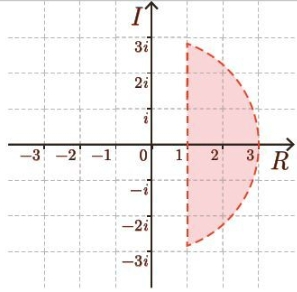
\includegraphics[scale=0.55]{dodatna_skica.jpeg}
    \end{figure}








\end{questions}



\end{document}